
\documentclass{../concepts/titul_protokol_p/prepareprotokol} %všechny balíčky pro protokol + titulní strana

\usepackage{graphicx}
\usepackage{newfloat}
\usepackage{caption}
\usepackage{booktabs}
\usepackage{amssymb}
\usepackage{amsmath}
\usepackage{newfloat}
\usepackage{caption}
\usepackage{siunitx}
\usepackage{textcomp}
\usepackage{comment}
\usepackage{gensymb}
\usepackage{subcaption}
\sisetup{inter-unit-product =$\cdot$}
%\sisetup{separate-uncertainty=true}

\praktikum{III} %číslo praktika (I, II nebo III)
\autor{David Němec} %jméno autora
\datum{17.\,3.\,2026} %datum měření
\cislo{30} %číslo úlohy
\nazev{Využití interference k měření tloušťky tenké vrstvy a~k~měření poloměrů křivosti čoček} %název úlohy

\DeclareFloatingEnvironment[fileext=los, placement={htbp}, name=Obrázek]{schema}

\newcommand{\nobars}{
Chybové úsečky nebyly pro~svou malou velikost pro~přehlednost vykresleny.}

\newcommand{\relative}[1]{
\frac{\sigma_{#1}}{#1}
}
\newcommand{\squared}[1]{
\left( #1 \right)^2
}
\newcommand{\relsqr}[1]{
\squared{\relative{#1}}
%\left( \frac{\sigma_{#1}}{#1} \right)^2
}

\begin{document}
\renewcommand{\figurename}{Graf}
\renewcommand{\refname}{Literatura}
\renewcommand{\today}{\number\day.\,\number\month.\,\number\year}

% add another graphics path to find ZPF.pdf for title page
% now searches for images in ./ and ../concepts/titul_protokol_p/
\graphicspath{{../concepts/titul_protokol_p/}}
\maketitle


% ========================== PRACOVNÍ ÚKOL ============================
\section{Pracovní úkol}
\begin{enumerate}
    \item Tolanského metodou změřte tloušťku tenké vrstvy ve dvou různých místech. Vyhodnoťte získané tloušťky a diskutujte, zda je vrstva v rámci chyby nepřímého měření na obou místech stejně silná.
    \item Pomocí Newtonových interferenčních kroužků změřte oba poloměry křivosti u dvou vybraných čoček zpracováním digitální fotografie.
    \begin{enumerate}
        \item Zkalibrujte mikroskop. Pořiďte digitální záznam kalibračního měřítka a zpracujte ho fitováním přímo v praktiku.
        \item Pořiďte digitální záznamy Newtonových kroužků pro jednotlivé povrchy čoček a zpracujte je fitováním přímo v praktiku.
        \item Výsledky měření porovnejte s poloměry křivosti měřených čoček uváděnými výrobcem.
        \item Z naměřených poloměrů křivosti spočítejte ohniskovou vzdálenost čoček a výsledky srovnejte s údaji uváděnými výrobcem. Materiál měřených čoček je optické sklo N-BK7, čočky nejsou tenké.
    \end{enumerate}
\end{enumerate}

% ============================= TEORIE ================================
\section{Teorie}
\subsection{Tolanského metoda měření tloušťky tenké vrstvy}

Schéma soustavy pro~měření tloušťky tenké vrstvy Tolanského metodou je znázorněno na~obrázku \ref{sch:tolansky}
a vznik interferenčních proužků na~klínové vzduchové mezeře pak~na~obrázku \ref{sch:klin}.
Do tenké vrstvy se~provede vryp a~následně se~horní část pokryje vysoce odrazivou krycí vrstvou
jako na~obrázku \ref{sch:vrypy}-b. Na~vzorek se~poté položí polopropustné zrcadlo tak, aby mezi zrcadlem
a~vzorkem vznikla klínová mezera s~malým úhlem klínu, a osvítí se monochromatickým světlem
o~vlnové délce $\lambda$ (v~této úloze světlo ze~sodíkové výbojky s~$\lambda_\mathrm{Na} = \qty{589.3}{\nm}$ \cite{vlnovedelky}).
Tím dojde k~interferenci na~klínu a~vzniku interferenčních proužků sledujících konstantní tloušťku vzduchové mezery.

Bez přítomnosti vrypu by~se~ve~vzdálenosti $x_2$ od $k$-tého proužku nacházel $(k+1)$-ní proužek.
Díky vrypu v~tenké vrstvě je však spodní rozhranní níže (právě o~tloušťku vrstvy $t$), což způsobí, že další
tmavý proužek vznikne již ve~vzdálenosti $x_2 - x_1$ od $k$-tého proužku. Interferenční proužky 
se~díky tomu deformují jako na~obrázku \ref{sch:vrypy}-a, v~zorném poli mikroskopu však byl u~této úlohy vidět
pouze jeden zlom. Z~geometrie a~interferenčních vlastností světla lze odvodit vztah 
pro~výpočet tloušťky vrstvy $t$ \cite{tolansky}:
\begin{equation}\label{eq:tloustka}
    t = \frac{x_1}{x_2} \frac{\lambda}{2}
\end{equation}

\begin{schema}[htbp]
    \centering
    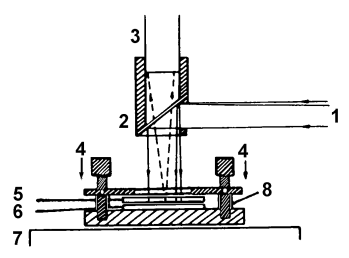
\includegraphics[width=0.5\linewidth]{tolansky.png}
    \caption{Schéma Tolanského metody:
    1 -- zdroj monochromatického světla (Na výbojka), 2 -- dělič svazku, 3 -- objektiv mikroskopu,
    4 -- stavěcí šrouby mechanického držáku, 5 -- polopropustné zrcadlo, 6 -- vzorek,
    7 -- stolek mikroskopu, 8 -- šrouby pro nastavení polopropustného zrcadla a vzorku \cite{tolansky}}
    \label{sch:tolansky}
\end{schema}

\begin{schema}[htbp]
    \centering
    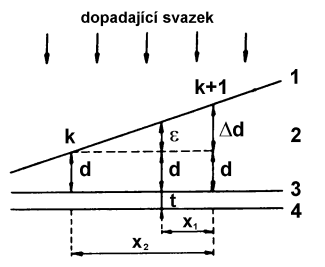
\includegraphics[width=0.5\linewidth]{klin.png}
    \caption{Vznik interferenčních proužků na klínové vzduchové mezeře:
    1 -- polopropustné zrcadlo, 2 -- vzduchová mezera (index lomu n = 1),
    3 -- horní plocha vrypu, 4 -- spodní plocha vrypu \cite{tolansky}}
    \label{sch:klin}
\end{schema}

\begin{schema}[htbp]
    \centering
    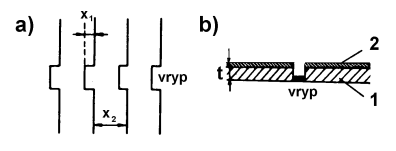
\includegraphics[width=0.5\linewidth]{vrypy.png}
    \caption{Schéma vrypu a vzniklých interferenčních proužků:
    (a) Obraz měřené vrstvy opatřené vrypem v~zorném poli mikroskopu.
    (b) Schematické znázornění této vrstvy:
    1 -- měřená vrstva s tloušťkou t, 2 -- krycí napařená vrstva reprodukující vrstvu s vrypem. \cite{tolansky}}
    \label{sch:vrypy}
\end{schema}

\subsection{Měření poloměru křivosti čoček pomocí Newtonových kroužků}

Pokud se na~čočku s~poloměrem křivosti $R$ položí planparalelní sklíčko a~osvítí se monochromatickým
světlem o~vlnové délce $\lambda$, dojde ke~vzniku interferenčních kroužků sledujících konstantní tloušťku
vzduchové mezery mezi čočkou a~sklíčkem. V~malé vzdálenosti $\rho$ od~středu čočky bude pro~tloušťku
vzduchové mezery přibližně platit \cite{newton}
\begin{equation}
    \label{eq:tloustkanarho}
    t(\rho) = \frac{\rho^2}{2 R} \,.
\end{equation}

Průběh intenzity světla ve vzdálenosti $\rho$ od středu čočky lze pak popsat funkcí \cite{newton}
\begin{equation}
    \label{eq:intenzita}
    I(\rho) = A \sin^2 \left[ \frac{2 \pi}{\lambda} \left( d + \frac{\rho^2}{2 R}\right)\right] + B \,,
\end{equation}
kde $A$ je amplituda intenzity, $B$ je intenzita pozadí a $d$ je dodatečná mezera mezi~čočkou
a~planparalelní destičkou způsobená různými nečistotami.

Ke správnému přepočtu mezi skutečnou vzdáleností a~vzdáleností v~pixelech na~digitálním záznamu
interferenčních kroužků je nutné pořídit také záznam kalibračního měřítka. Černé čárky označující
jednotlivé dílky se~na~záznamu intenzity projeví ostrými skoky, které lze popsat funkcí ve~tvaru \cite{newton}
\begin{equation}
    \label{eq:meritko}
    I(x) = A \left\lfloor \frac{x}{T} - x_0 + s - \left\lfloor \frac{x}{T} - x_0 \right\rfloor \right\rfloor + B \,,
\end{equation}
kde $\lfloor a \rfloor$ označuje dolní celou část čísla $a$, $A$ je amplituda intenzity, $B$ je intenzita pozadí,
$T$ je perioda (tedy počet pixelů na jeden dílek kalibračního měřítka), $x$ je souřadnice aktuálního pixelu,
$x_0$ je souřadnice počátku a $s$ je střída
(určuje jakou část periody je skoková funkce rovna jedné).


\subsection{Ohnisková vzdálenost tlusté čočky}

Je-li prostředí před~i~za~čočkou stejné s~indexem lomu $n=1$, lze ohniskovou vzdálenost 
$f$ tlusté čočky vypočítat jako
\begin{equation}
    \label{eq:ohniskovavzdalenost}
    f = \frac{n}{n-1} \frac{R_1 R_2}{n (R_2 - R_1) + (n-1) d} \,,
\end{equation}
kde $n$ je index lomu čočky, $R_1$ a $R_2$ jsou poloměry křivosti přední a~zadní lámavé plochy čočky
a~$d$ je tloušťka čočky v~místě optické osy (ve~středu čočky) \cite{wiki}.

\subsection{Měřicí přístroje a jejich nejistoty}
\begin{enumerate}
    \item \textbf{Mikroskop PZO se stupnicí}:
    
    Mikroskop byl použit k~měření tloušťky tenké vrstvy Tolanského metodou. Stupnice mikroskopu
    umožnovala měřit s~přesností na~0.01 dílku velké stupnice (skutečný fyzikální rozměr není důležitý).
    Vzhledem k~tomu, že interferenční proužky nebyly zcela ostré, odhaduji nejistotu hodnoty na~stupnici
    jako 0.05 dílku velké stupnice.

    \item \textbf{Mikroskop Motic BA310}:
    
    Tento mikroskop byl připojen ke~kameře a~použit k~pořízení digitálních záznamů Newtonových kroužků.
    Kalibrace (přepočet počtu pixelů na~skutečnou délku) byla provedena nasnímáním kalibračního měřítka.
    Použita byla hrubá stupnice měřítka s~dílkem \qty{0.1}{\mm}.

\end{enumerate}


% ======================== VÝSLEDKY MĚŘENÍ ===========================
\section{Výsledky měření}

\subsection{Měření tloušťky tenké vrstvy Tolstého metodou}

Nejprve byl pod~mikroskopem se~stupnicí pozorován vzorek tenké vrstvy s~vrypem, osvícený sodíkovou výbojkou o~vlnové
délce $\lambda_\mathrm{Na} = \qty{589.3}{nm}$ \cite{vlnovedelky}. Na~třech různých místech vzorku byly
změřeny pozice tmavých interferenčních proužků vůči stupnici mikroskopu. Pro~kontrolu byly na~třetím místě
proměřeny dva sousední proužky (označil jsem je jako $3$ a $3'$). Vždy byla určena jen pozice pravého 
kraje tmavého proužku, jelikož byla nejlépe čitelná. 

Vzdálenost $x_1$ je podle obrázku \ref{sch:vrypy}-a rovna
rozdílu pozic tmavého proužku před~vrypem ($x_{1l}$) a toho samého proužku za~vrypem ($x_{1r}$), zatímco $x_2$
se určí jako rozdíl pozic dvou sousedních proužků ($x_{2r}$ a $x_{2l}$).
Protože ve~výpočtu tloušťky $t$
podle vztahu (\ref{eq:tloustka}) jsou vzdálenosti $x_1$ a~$x_2$ v~poměru, není nutné znát skutečné
fyzikální jednotky těchto vzdáleností, stačí uvažovat jen jejich relativní velikost vzhledem
k~dílkům velké stupnice mikroskopu (označeným d.m.).

Naměřené pozice pravých okrajů tmavých interferenčních proužků vůči stupnici mikroskopu a~z~nich vypočtené
tloušťky vzorku jsou uvedeny v tabulce \ref{tab:tloustky}. Nejistota určení tloušťky byla podle \cite{englich}
vypočtena jako
\begin{equation}
    \label{eq:sigmat}
    \sigma_t = t \sqrt{\relsqr{x_1} + \relsqr{x_2}} \,,
\end{equation}
kde $\sigma_{x_1} = \sigma_{x_2} = \sqrt{2} \sigma_x = \sqrt{2} \cdot 0.05 \, (\mathrm{d.m.})$ jsou nejistoty
vzdáleností $x_1$ resp. $x_2$ dané nejistotou určení pozice okraje proužku $\sigma_x = 0.05 \,(\mathrm{d.m.})$.


\begin{table}[!htbp]
\centering
\caption{Pozice interferenčních proužků a~z~nich vypočtené tloušťky tenké vrstvy. Jednotka d.m.
je dílek velké stupnice mikroskopu.}
\begin{tabular}{cccccccc}
 \toprule
 místo & $x_{1l}\, (\mathrm{d.m.})$ & $x_{1r}\, (\mathrm{d.m.})$ & 
 $x_{1r}\, (\mathrm{d.m.})$ & $x_{2l}\, (\mathrm{d.m.})$ & 
 $x_{2r}\, (\mathrm{d.m.})$ & $x_{2r}\, (\mathrm{d.m.})$ & $t \, (\unit{\micro \meter})$\\
 \midrule
 $1$ & $2.83(5)$ & $5.74(5)$ & $2.91(7)$ & $2.83(5)$ & $4.44(5)$ & $1.61(7)$ & $0.53(3)$ \\
 $2$ & $3.49(5)$ & $4.80(5)$ & $1.31(7)$ & $3.49(5)$ & $4.88(5)$ & $1.39(7)$ & $0.28(2)$ \\
 $3$ & $4.32(5)$ & $5.80(5)$ & $1.48(7)$ & $4.32(5)$ & $6.58(5)$ & $2.26(7)$ & $0.193(11)$ \\
 $3'$ & $1.97(5)$ & $3.47(5)$ & $1.50(7)$ & $1.97(5)$ & $4.35(5)$ & $2.38(7)$ & $0.186(10)$ \\
 \bottomrule
\end{tabular}
\label{tab:tloustky}
\end{table}

V místě $3$ tedy podle tabulky \ref{tab:tloustky} uvažuji tloušťku $0.19(1) \unit{\micro\meter}$.

%=======================================
\subsection{Měření poloměrů křivosti čoček pomocí Newtonových kroužků}

Ve~druhém úkolu byla studována interference na~klínové mezeře mezi zakřivenou lámavou plochou čočky
a~planparalelní skleněnou destičkou.
Ke zjištění poloměrů křivosti čoček byl použit digitální záznam obrazu z~mikroskopu (obrázek 
\ref{sch:fotky}) a~následně 
zpracování pomocí programu Origin. Obraz byl rozdělen do~tří kanálů (červený, zelený a modrý), přičemž
pro~kalibraci byl využit zelený kanál a pro~analýzu interferenčních kroužků od~čoček byl použit červený kanál.
Průběh intenzity v~daném barevném kanálu ve~vodorovném řezu byl během kalibrace fitován předpřipravenou funkcí
\texttt{Scale} (ve~tvaru (\ref{eq:meritko})) a~poté během analýzy Newtonových kroužků funkcí \texttt{NewtonRings}
(ve~tvaru (\ref{eq:intenzita})). Některé parametry (např. amplituda a intenzita pozadí) navíc
nebyly uvažovány jako konstantní, ale byly opatřeny lineární a~kvadratickou korekcí na~vzdálenost od~středu
digitálního záznamu. Průběhy intenzit s~nafitovanými parametry funkcí \texttt{Scale}
a~\texttt{Newtonrings} jsou vykresleny na~obrázcích \ref{fig:fit_meritko}, \ref{fig:fit_cockaf50} 
a~\ref{fig:fit_cockaf100}.

% ========================== fotky z mikroskopu
\begin{schema}[!htbp]
    \centering
    \begin{subschema}{\textwidth}
        \centering
        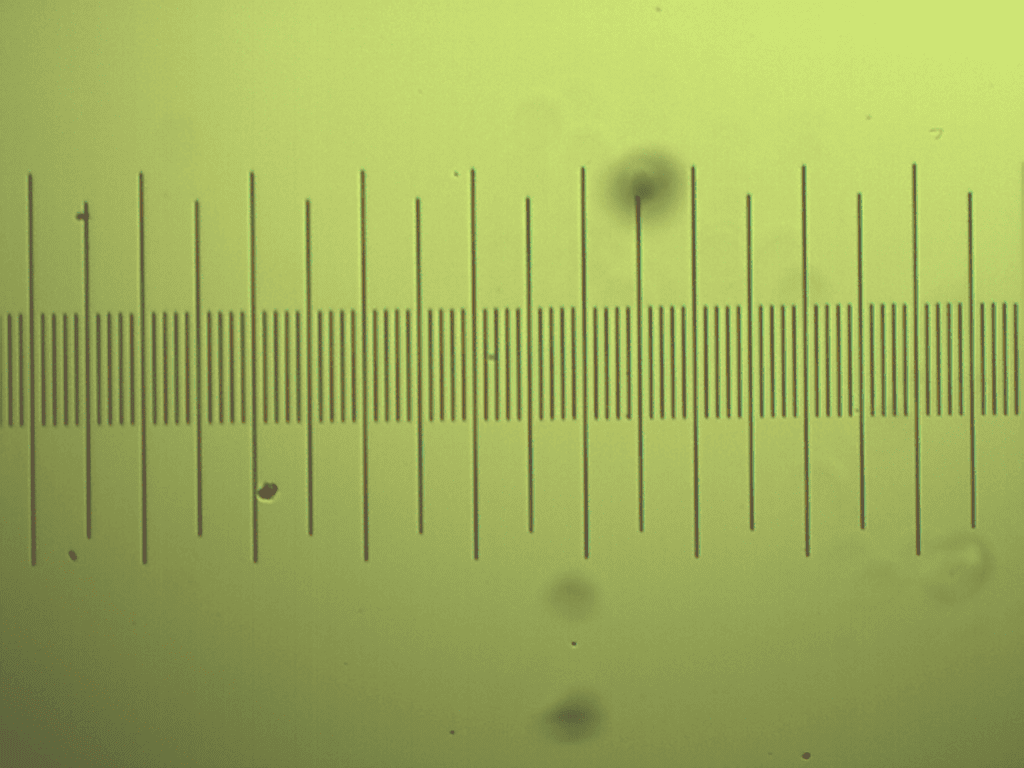
\includegraphics[width=0.3\textwidth]{obr_meritko.png}
        \caption{Kalibračního měřítko.}
        \label{obr_meritko}
    \end{subschema}

    \vspace{3mm}

    \begin{subschema}{0.45\textwidth}
        \centering
        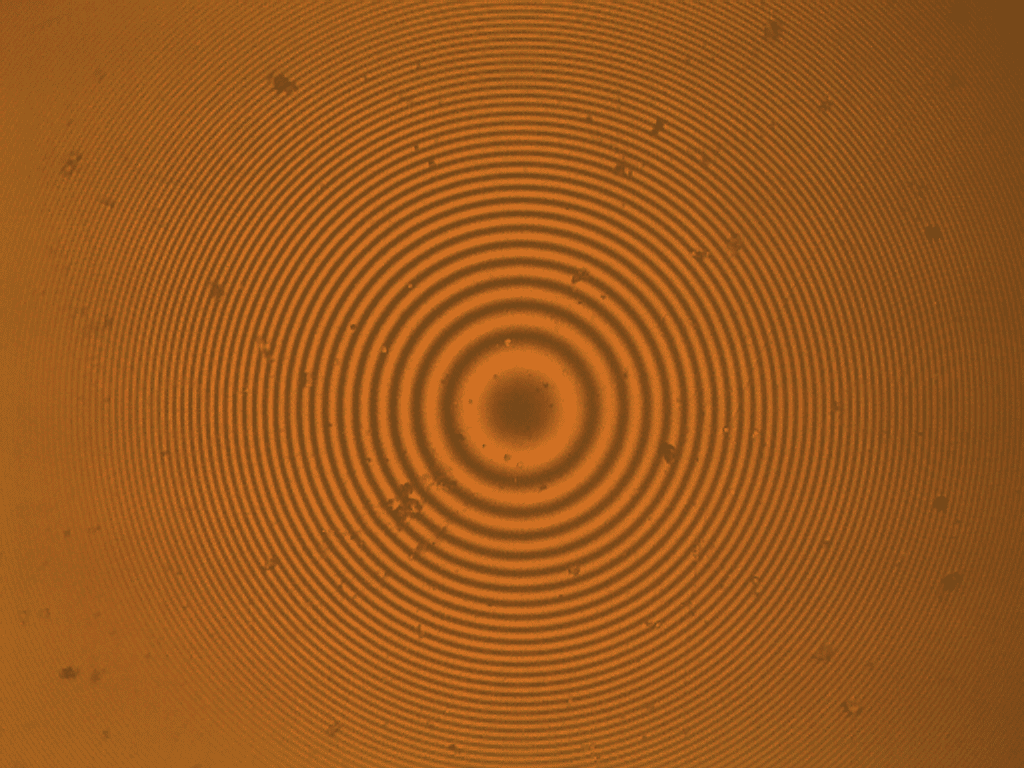
\includegraphics[width=0.5\linewidth]{obr_f50plus.png}
        \caption{Čočka F50: vypuklé rozhranní.}
        \label{obr_f50plus}
    \end{subschema}
    \hfill
    \begin{subschema}{0.45\textwidth}
        \centering
        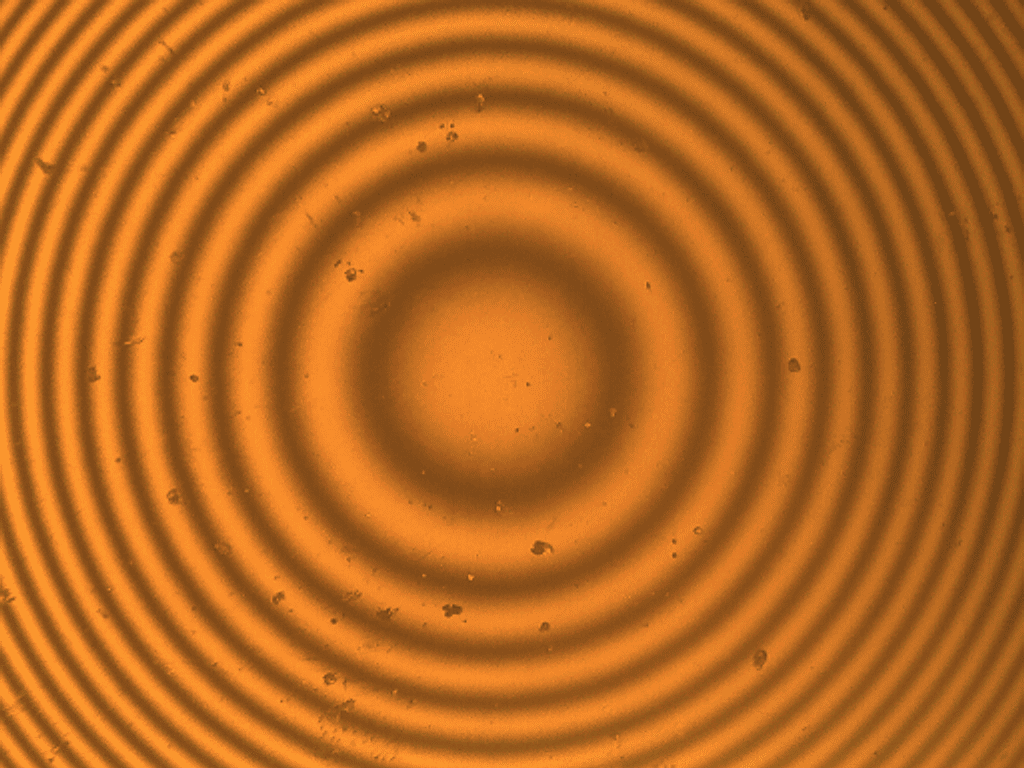
\includegraphics[width=0.5\linewidth]{obr_f50minus.png}
        \caption{Čočka F50: vyduté rozhranní.}
        \label{obr_f50minus}
    \end{subschema}

    \vspace{3mm}

        \begin{subschema}{0.45\textwidth}
        \centering
        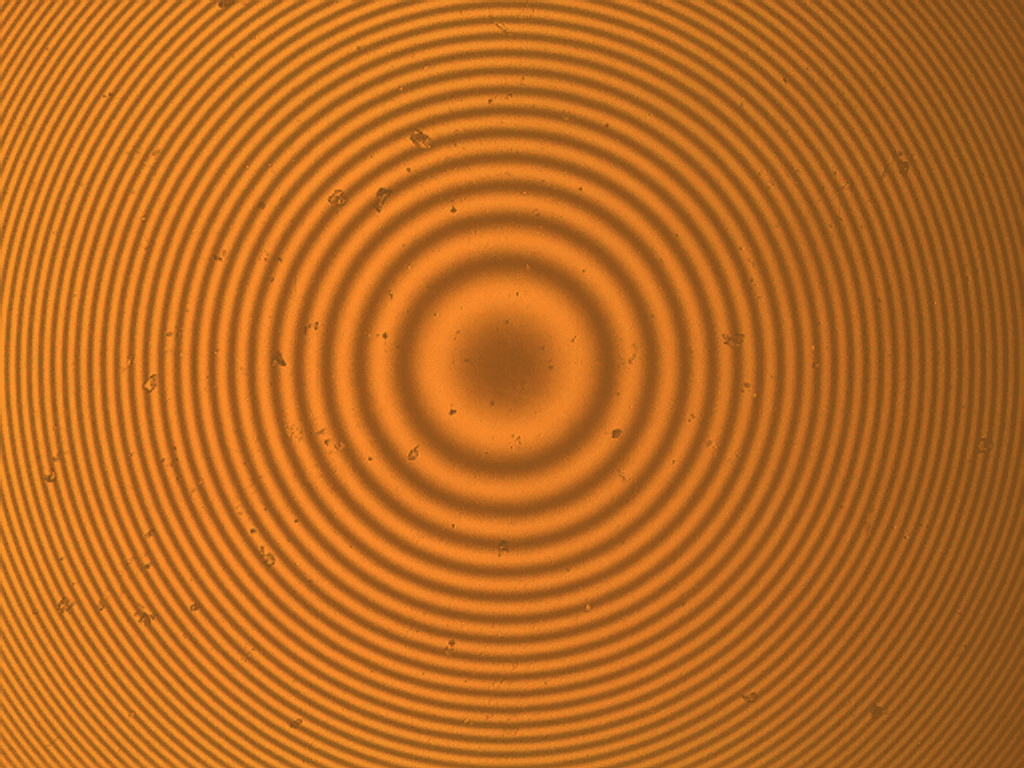
\includegraphics[width=0.5\linewidth]{obr_f100plus.png}
        \caption{Čočka F100: vypuklé rozhranní.}
        \label{obr_f100plus}
    \end{subschema}
    \hfill
    \begin{subschema}{0.45\textwidth}
        \centering
        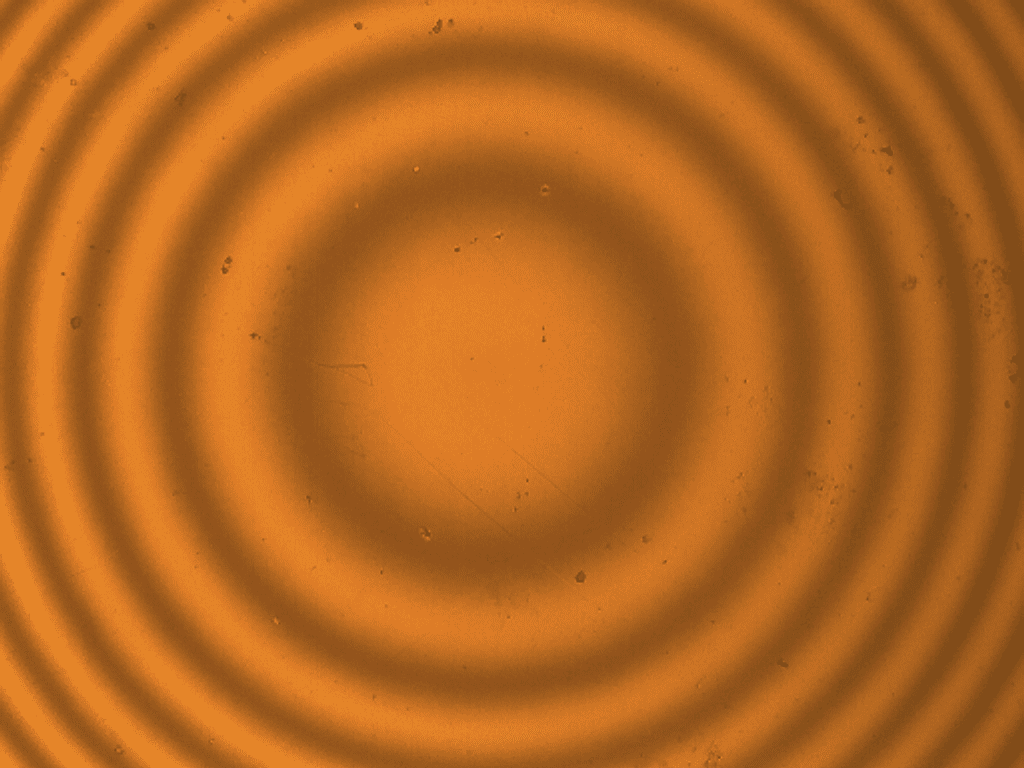
\includegraphics[width=0.5\linewidth]{obr_f100minus.png}
        \caption{Čočka F100: vyduté rozhranní.}
        \label{obr_f100minus}
    \end{subschema}

    \caption{Digitální záznamy kalibračního měřítka a Newtonových kroužků.}
    \label{sch:fotky}
\end{schema}

%================================== fity z Originu
\begin{figure}[!htbp]
    \centering
    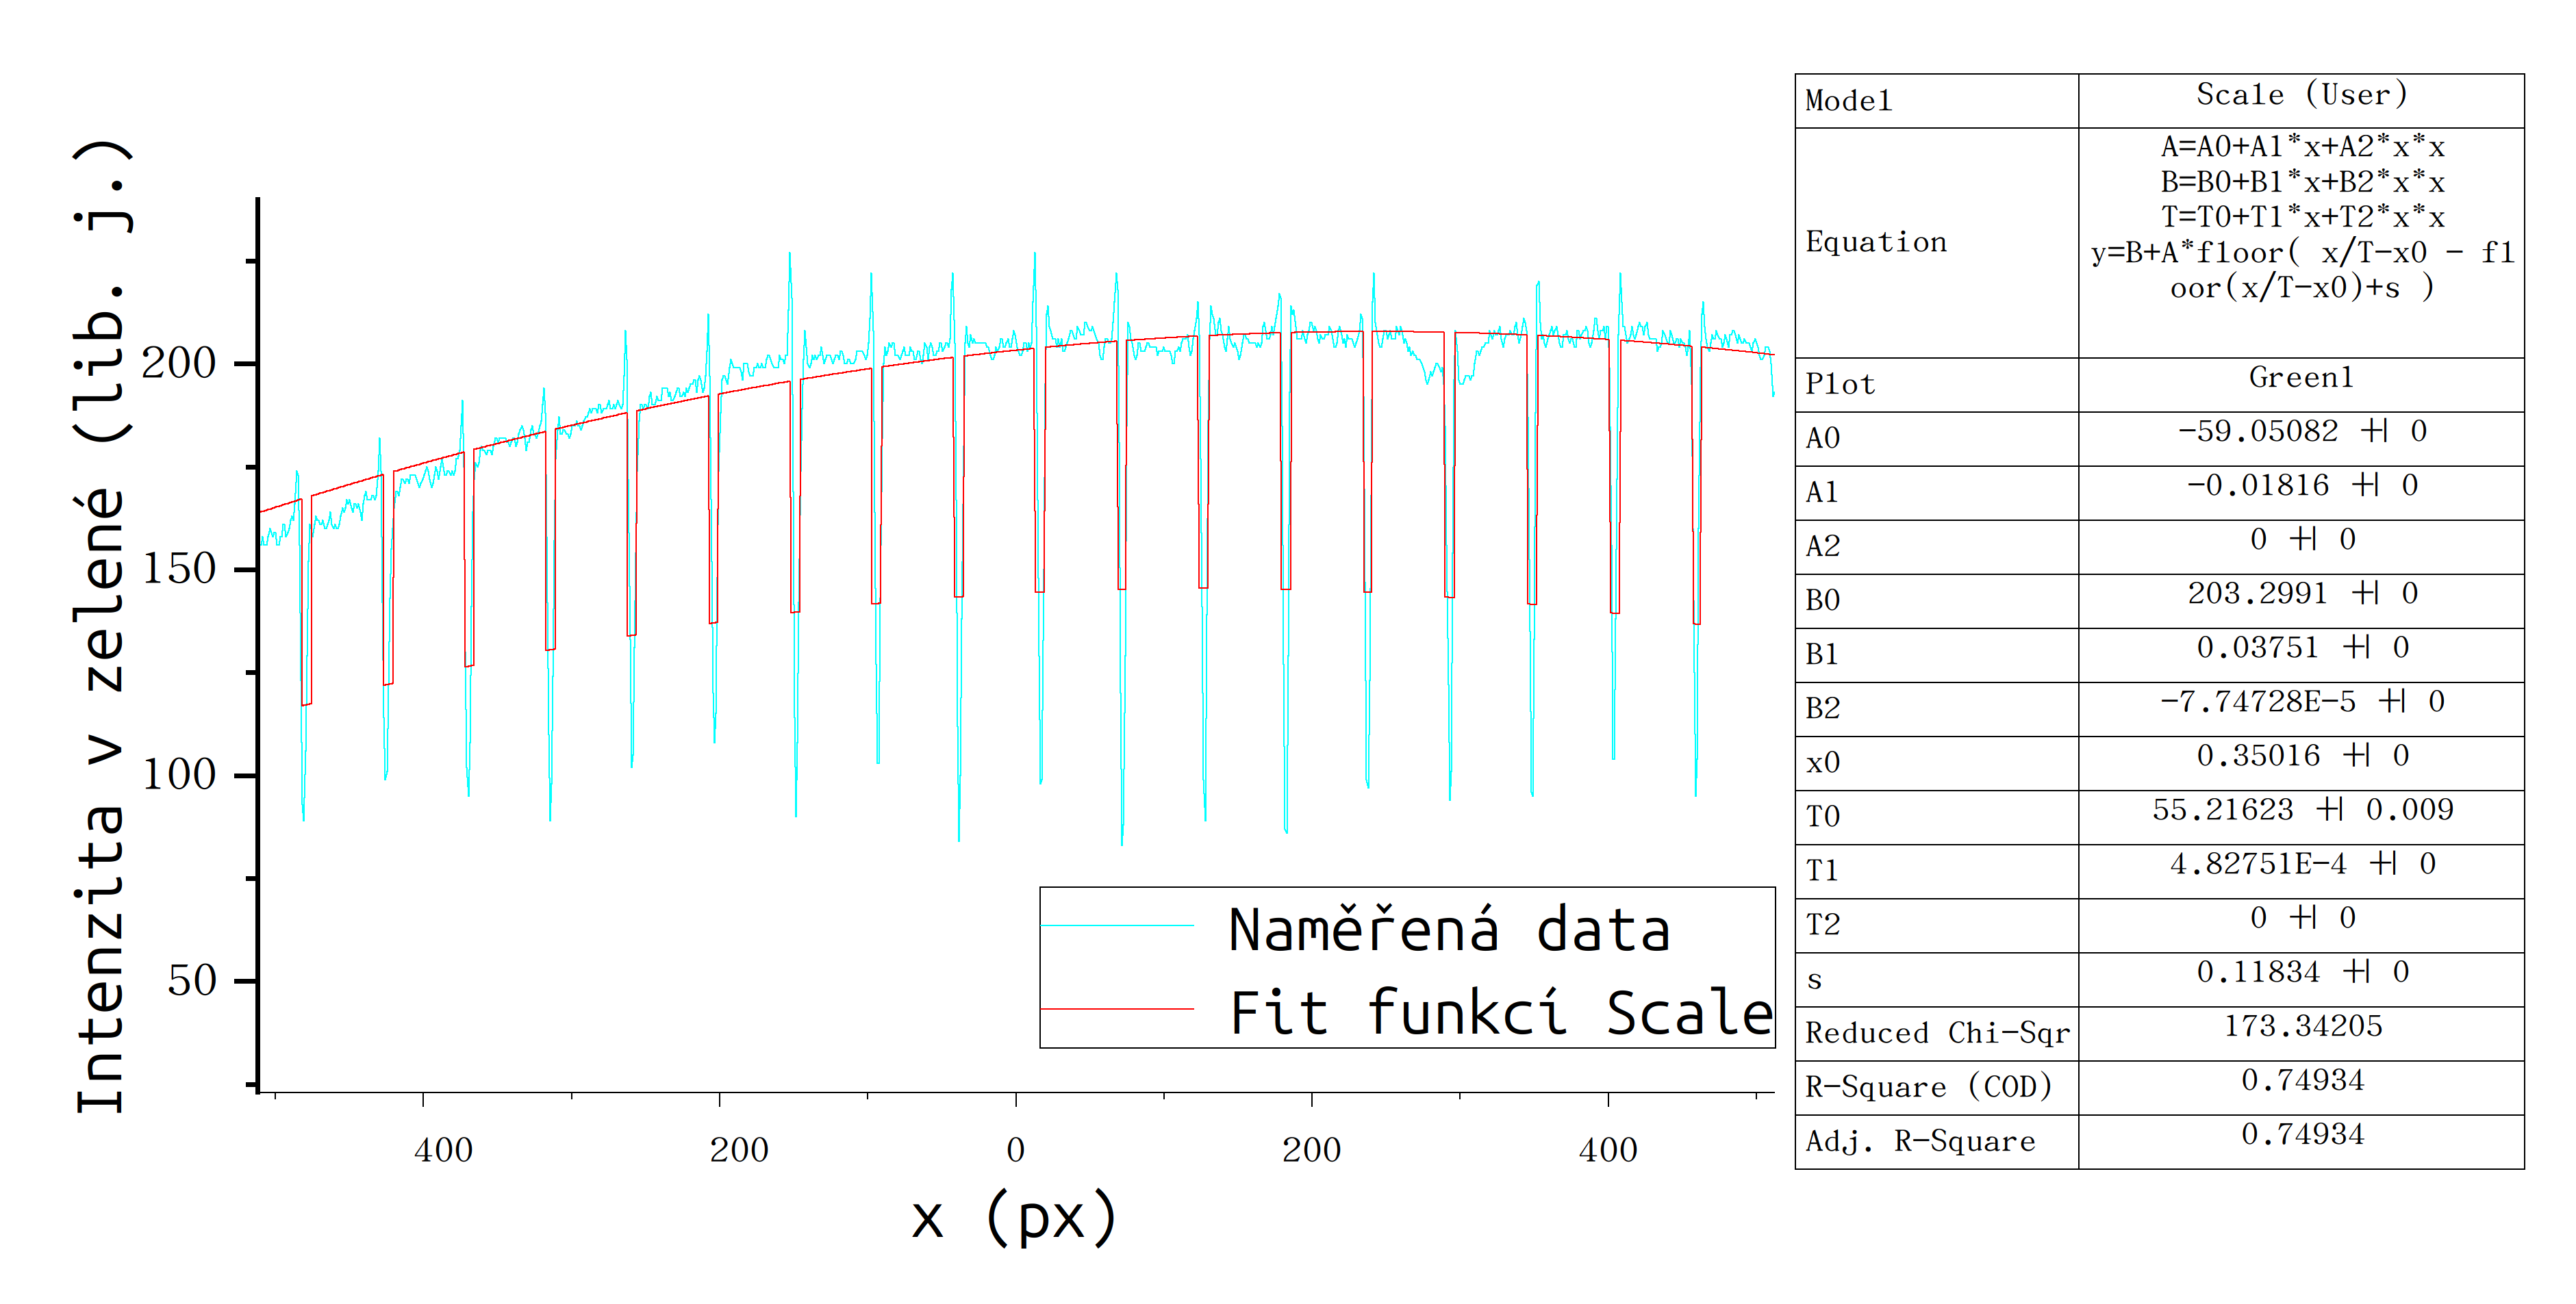
\includegraphics[width=0.8\linewidth]{meritko.png}
    \caption{Fitovaný intenzitní profil v zeleném kanálu pro kalibrační měřítko.}
    \label{fig:fit_meritko}
\end{figure}

\begin{figure}[!htbp]
    \centering
    \begin{subfigure}{\textwidth}
        \centering
        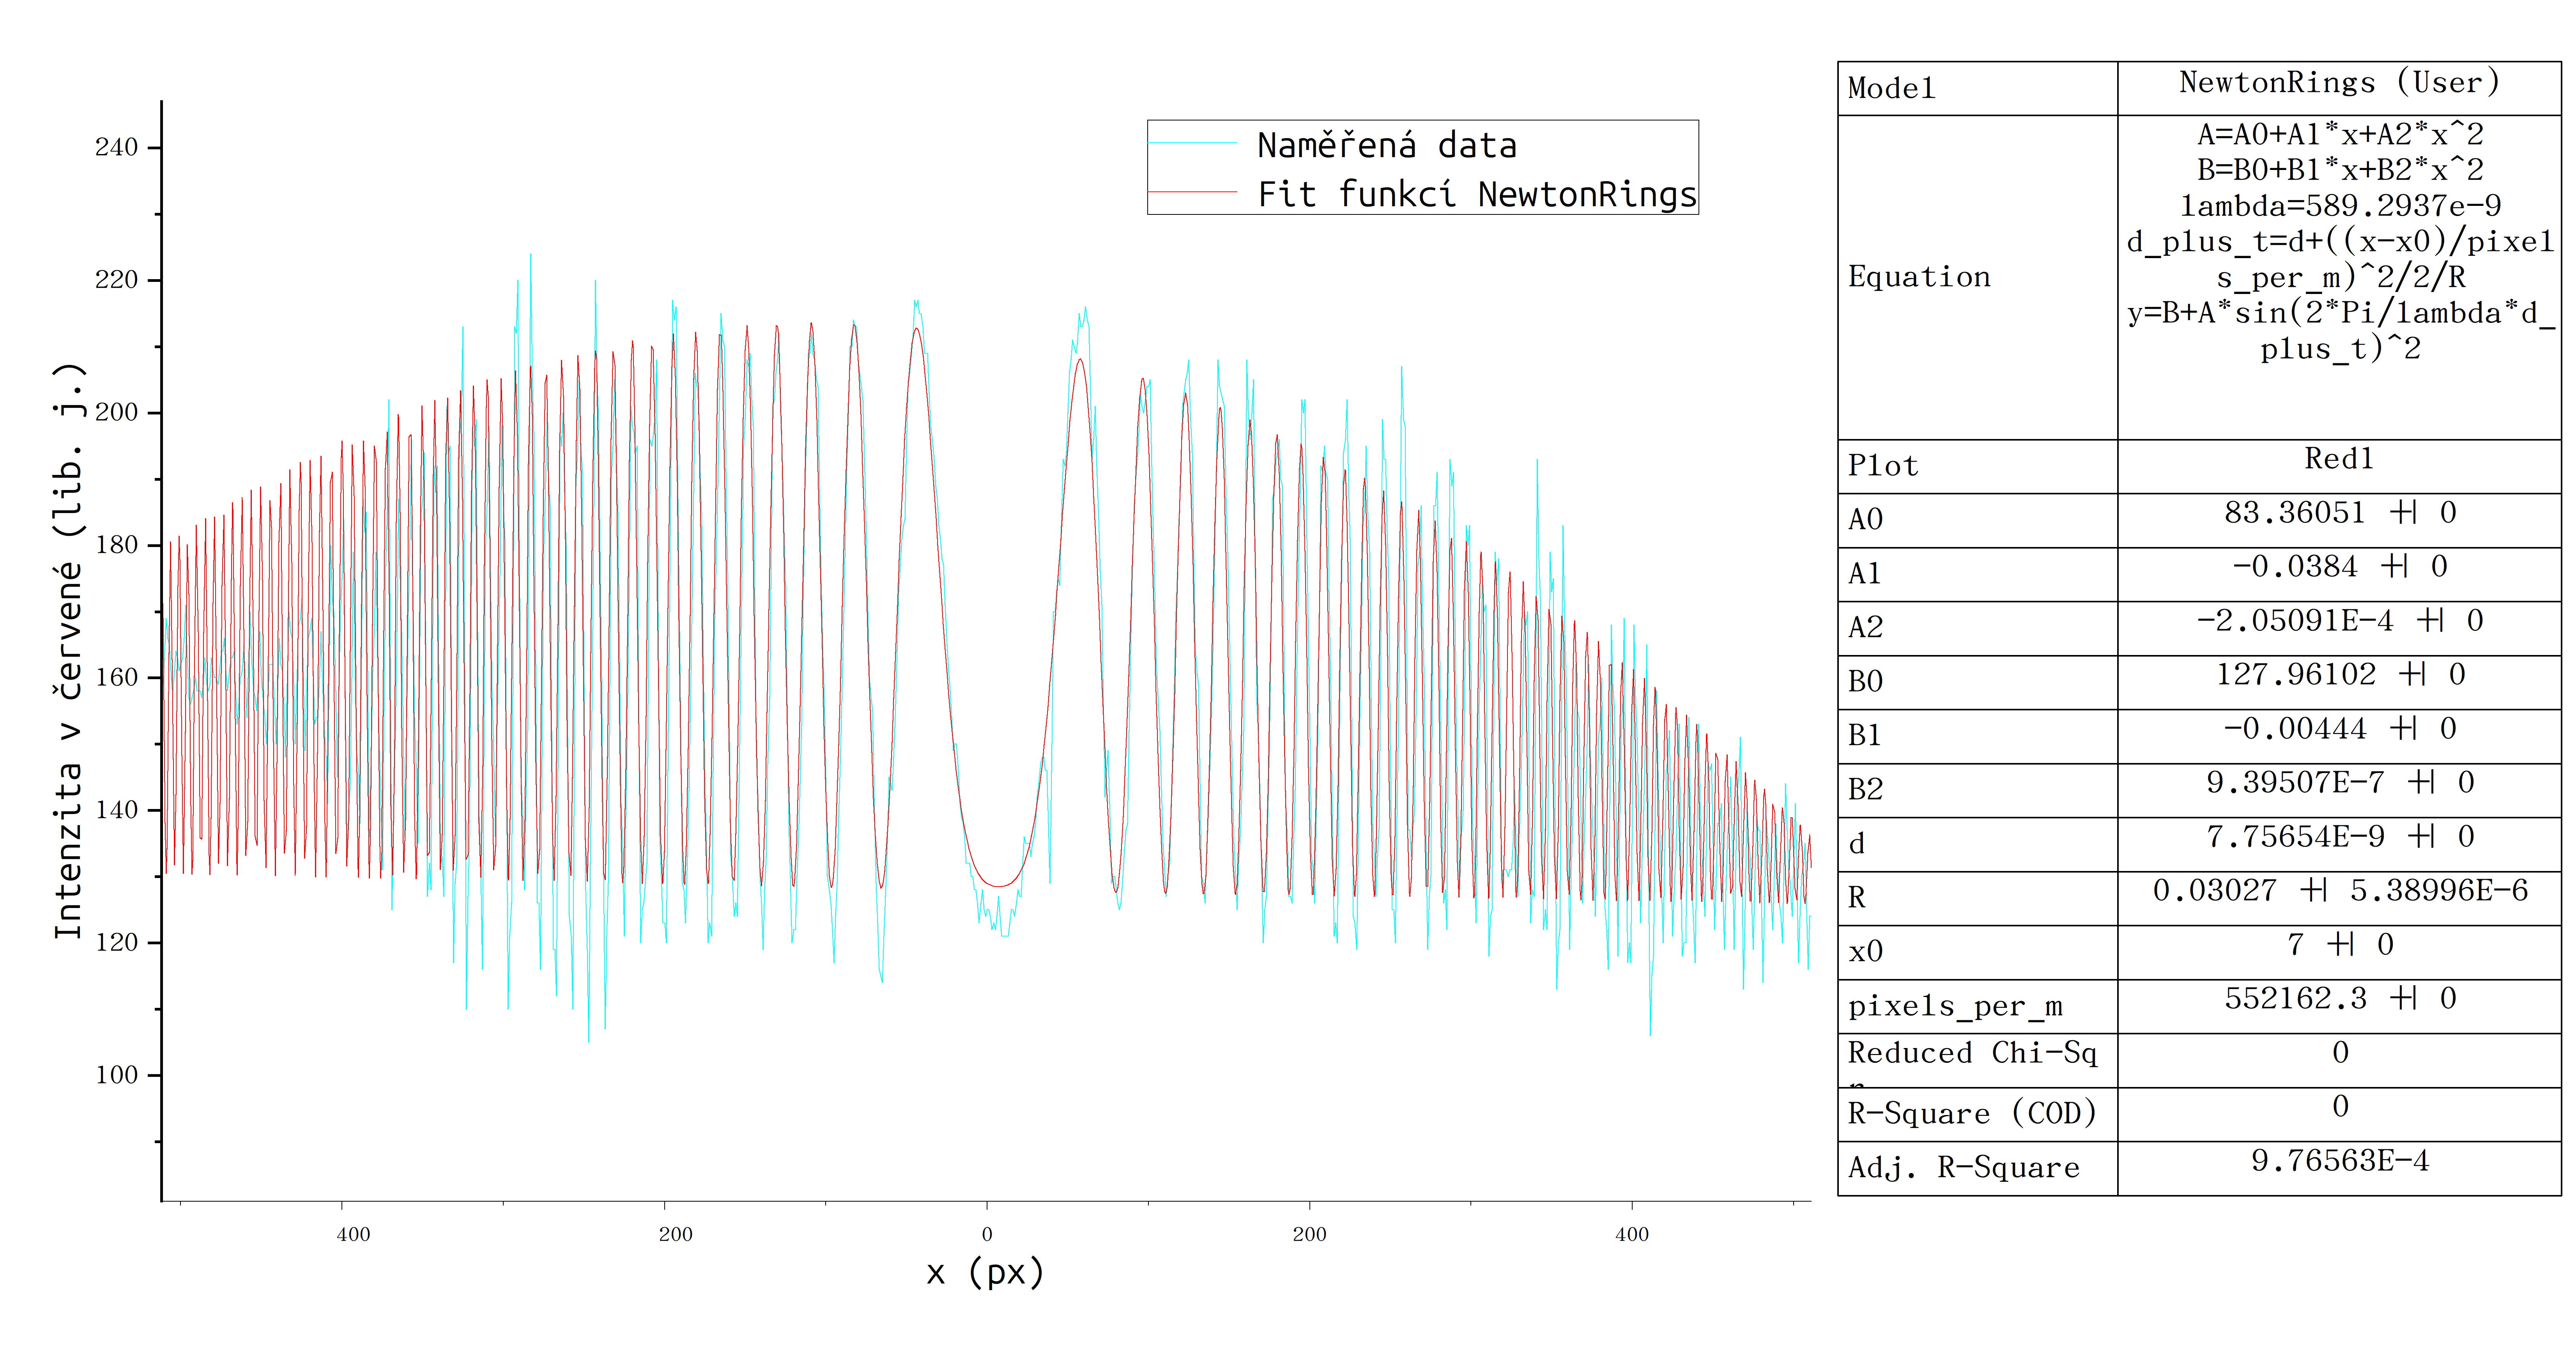
\includegraphics[height=8cm]{f50plus.png}
        \caption{Čočka F50: vypuklé rozhranní.}
    \end{subfigure}
    
    \begin{subfigure}{\textwidth}
        \centering
        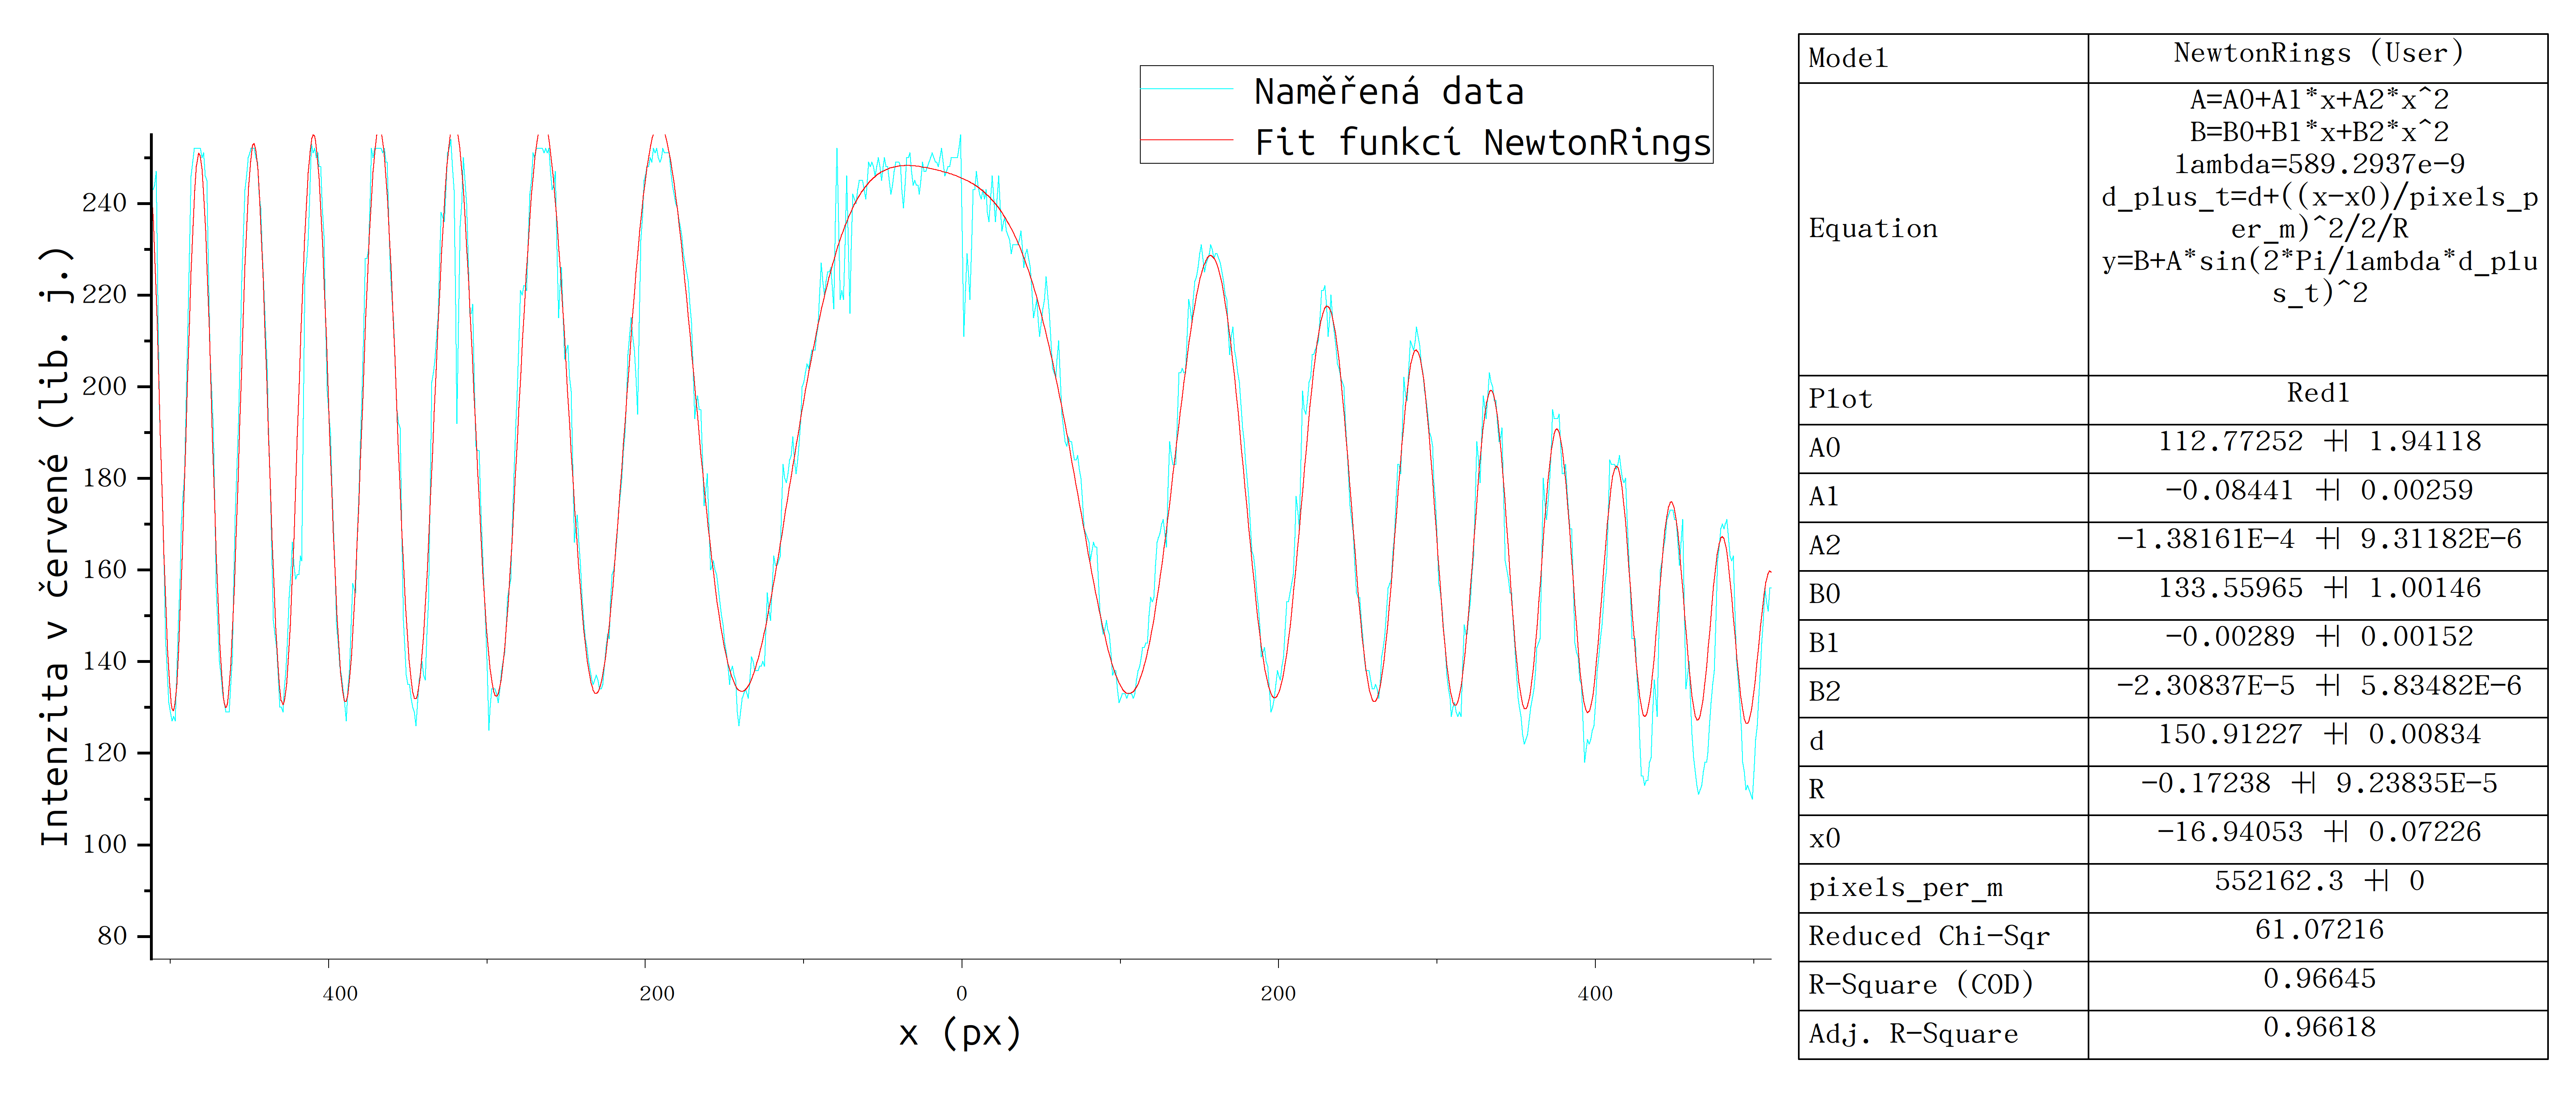
\includegraphics[height=6cm]{f50minus.png}
        \caption{Čočka F50: vyduté rozhranní.}
    \end{subfigure}
    \caption{Fitované intenzitní profily v červeném kanálu pro čočku F50.}
    \label{fig:fit_cockaf50}
\end{figure}

\begin{figure}[!htbp]
    \begin{subfigure}{\textwidth}
        \centering
        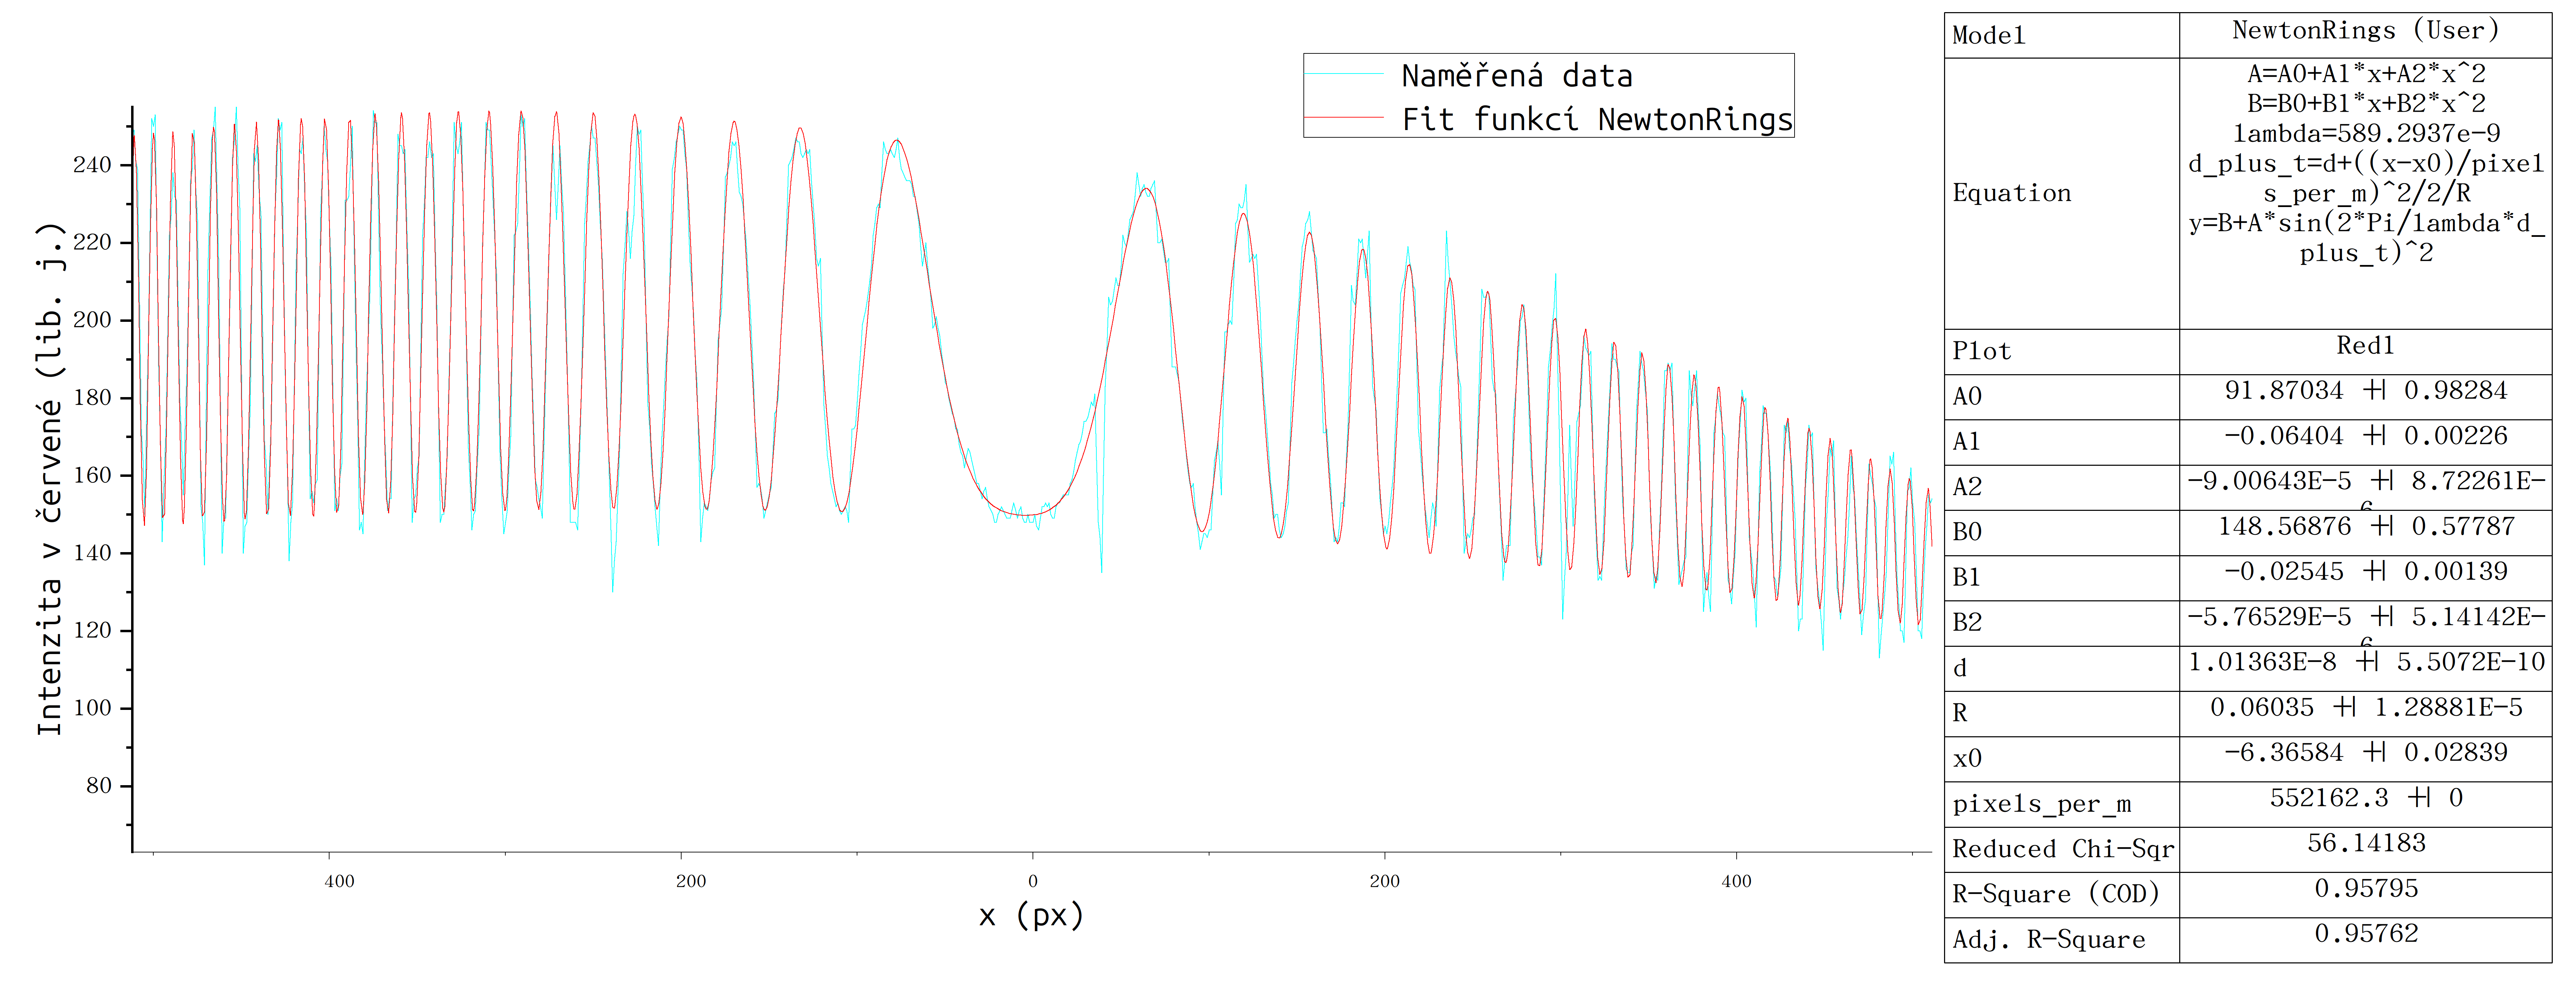
\includegraphics[height=6cm]{f100plus.png}
        \caption{Čočka F100: vypuklé rozhranní.}
    \end{subfigure}
    
    \begin{subfigure}{\textwidth}
        \centering
        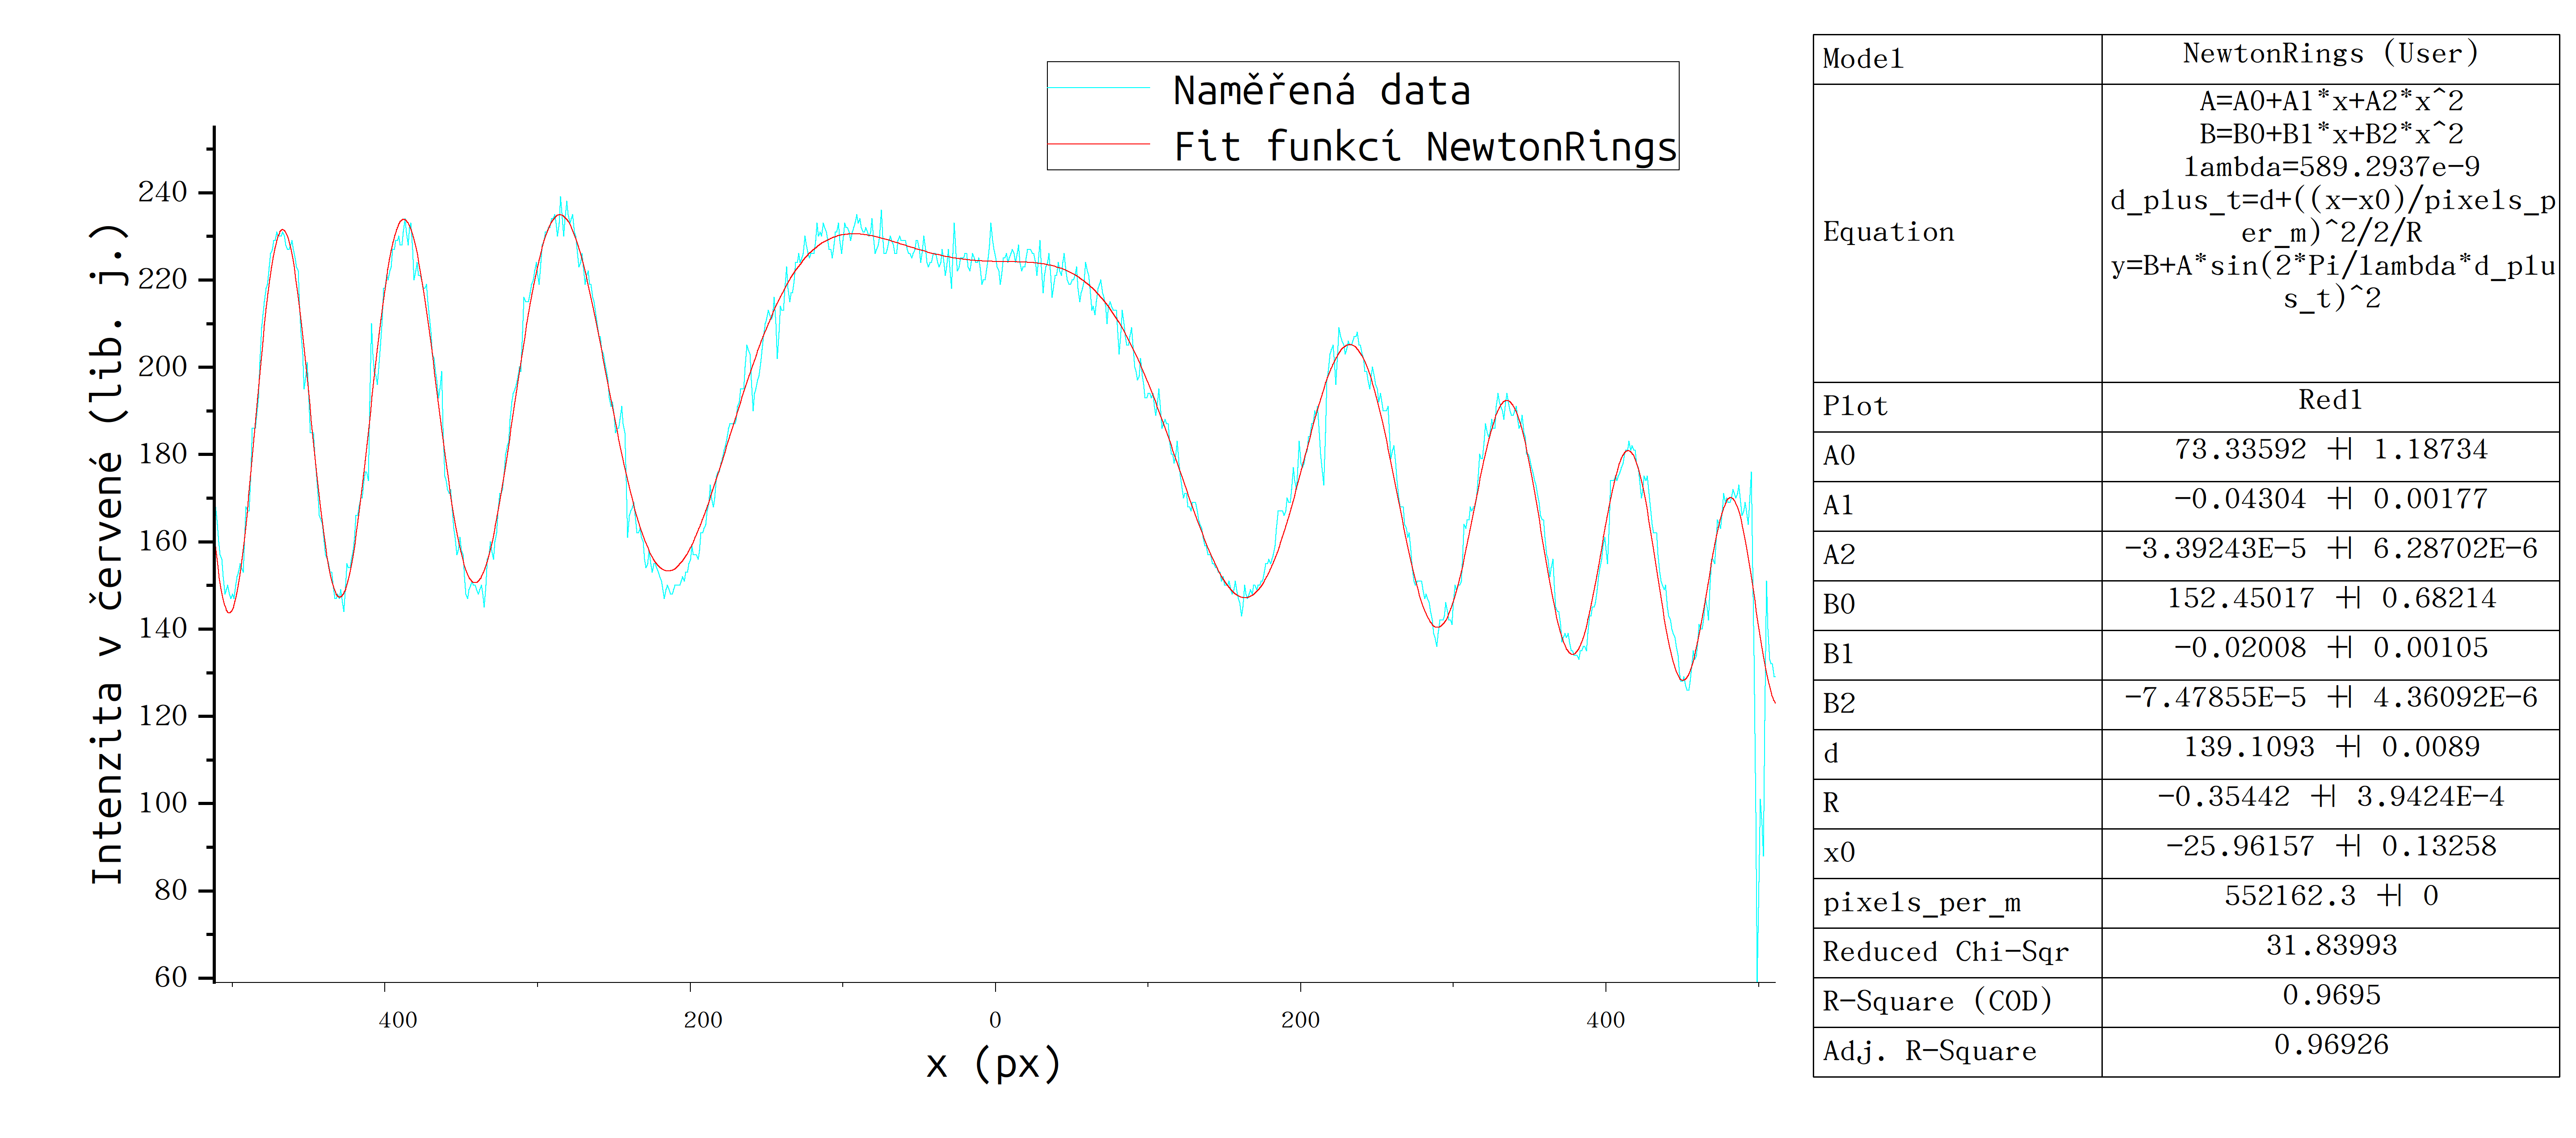
\includegraphics[height=6cm]{f100minus.png}
        \caption{Čočka F100: vyduté rozhranní.}
    \end{subfigure}
    \caption{Fitované intenzitní profily v červeném kanálu pro čočku F100.}
    \label{fig:fit_cockaf100}
\end{figure}

Hlavním parametrem získaným z~fitu kalibrace je přepočet mezi~pixely obrazu
a~skutečnou jednotkou vzdálenosti $T_0$. Ten byl určen jako $T_0 = 552.16(9) \, \mathrm{px\,mm^{-1}}$.
V~jednotkách $\mathrm{px\,m^{-1}}$ byl následně dosazován jako pevný parametr funkce \texttt{NewtonRings}.
Hlavním výstupním parametrem z~fitu interferenčních kroužků čoček byly poloměry křivosti jednotlivých lámavých
ploch čoček. Kladný poloměr lámavé plochy, kde je čočka vypuklá, značím $R_1$ a~záporný poloměr, kde je čočka
vydutá, značím $R_2$.

Výsledné poloměry křivosti i~s~jejich nejistotami a~srovnání s~poloměry křivosti udávanými výrobcem jsou v~tabulce
\ref{tab:polomery}. Nejistota poloměru křivosti nebyla upravováva o~nejistotu kalibrace, jelikož ta byla řádově
menší (viz Diskuzi).

\begin{table}[!htbp]
    \centering
    \caption{Experimentálně určené poloměry křivosti obou čoček a~srovnání s~hodnotami udávanými výrobcem.}
    \begin{tabular}{c|cc|cc}
        \toprule
         & \multicolumn{2}{c|}{experimentální} & \multicolumn{2}{c}{tabulkové} \\
        \midrule
        čočka & $R_{1} \, (\mathrm{mm})$ & $R_{2} \, (\mathrm{mm})$ & 
        $R_{1} \, (\mathrm{mm})$ & $R_{2} \, (\mathrm{mm})$ \\
        \midrule
        F50 & $30.270(5)$ & $-172.38(9)$ & $30.06$ & $-172.0$ \\
        F100 & $60.350(13)$ & $-354.4(4)$ & $60.02$ & $-353.30$ \\
        \bottomrule
    \end{tabular}
    \label{tab:polomery}
\end{table}

%==================================================
\subsection{Určení ohniskové vzdálenosti čoček}

Výrobce udává, že obě čočky jsou vyrobené z~optického skla N-BK7, které má pro vlnovou délku 
$\lambda_\mathrm{Na} = \qty{589.3}{nm}$ \cite{vlnovedelky} index lomu $n = 1.51673$ \cite{schott}.
Z indexu lomu, tlouštěk čoček (udávaných výrobcem, dostupných v~pokynech u~úlohy) a~naměřených poloměrů 
křivosti čoček byly nakonec podle vztahu (\ref{eq:ohniskovavzdalenost})
vypočteny jejich ohniskové vzdálenosti. V tabulce \ref{tab:cockyvysledky} jsou uvedeny tabulkové tloušťky,
tabulkové ohniskové vzdálenosti a~experimentálně určené ohniskové vzdálenosti zkoumaných čoček. Nejistota
ohniskové vzdálenosti byla vypočtena podle \cite{englich} jako
\begin{equation}
    \label{eq:sigmaf}
    \sigma_f = \frac{n |R_2|}{n-1} \frac{\sqrt{\left[ n (R_2 - R_1) + (n-1) d + n R_1 R_2 \right]^2 \sigma_{R_1}^2 +
    \left[ n (R_2 - R_1) + (n-1) d - n R_1 R_2 \right]^2 \sigma_{R_2}^2 }}
    {\left[ n (R_2 - R_1) + (n-1) d \right]^2} \,,
\end{equation}
přičemž nejistoty indexu lomu a tlouštěk čoček neuvažuji.


\begin{table}[!htbp]
    \centering
    \caption{Tloušťky čoček a jejich tabulkové i experimentálně určené ohniskové vzdálenosti.}
    \begin{tabular}{cccc}
        \toprule
        čočka & $d \, (\mathrm{mm})$ & $f_\mathrm{tab} \, (\mathrm{mm})$ & $f_\mathrm{exp} \, (\mathrm{mm})$ \\
        \midrule
        F50 & $6.5$ & $50.0$ & $50.380(11)$ \\
        F100 & $4.0$ & $100.0$ & $100.13(3)$ \\
        \bottomrule
    \end{tabular}
    \label{tab:cockyvysledky}
\end{table}

% ============================ DISKUZE ===============================
\section{Diskuze}

\textit{Měření tloušťky tenké vrstvy.}
Tloušťka tenké vrstvy byla na~třech místech změřena jako $\qty{0.53(3)}{nm}$, $\qty{0.28(2)}{nm}$
a~$\qty{0.19(1)}{nm}$ s~relativními nejistotami $6\,\%$, $7\,\%$ a $5\,\%$. Ty jsou dané především nejistotou
určení pozice bodů vůči stupnici mikroskopu. Kvůli neostrosti interferenčních proužků se~jejich okraj,
a~tím i~jejich vzdálenost, nedala určit dostatečně přesně. Jinak však mikroskop umožnoval odečítat pozice
se~zrhuba pětinásobnou přesností. Hodnoty tloušťky se~na~různých místech liší o~více než několik standardních
nejistot, lze tedy s~jistotou tvrdit, že vrstva má proměnnou tloušťku. Pro~kontrolu, že nedošlo ke~hrubé chybě
nebo že nejistota nebyla přeci jen podceněna, byl ve~třetím místě proměřen i~vedlejší interferenční proužek.
V~rámci nejistoty se~v~tomto místě obě hodnoty tloušťky shodují, hrubou chybu lze tedy vyloučit.

Předpokládám, že tloušťka vzorku je menší než vlnová délka použité sodíkové výbojky 
$\lambda_\mathrm{Na} = \qty{589.3}{nm}$ \cite{vlnovedelky}. Jinak by~bylo nutné použít ještě jiný
monochromatický zdroj o~jiné vlnové délce, protože by hodnota tloušťky nebyla jednoznačná. Tloušťky lišící
se~o~celočíselné násobky vlnové délky totiž nelze rozlišit při~provedení experimentu pouze s~jednou
vlnovou délkou.

%============================
\textit{Kalibrace mikroskopu pro analýzu Newtonových kroužků.}
Před vlastním zkoumáním Newtonových kroužků čoček bylo nutné zkalibrovat mikroskop s~digitálním záznamem, tedy
především určit hodnotu přepočtu mezi vzdáleností v~pixelech a~skutečnou vzdáleností. K~tomu byl pořízen
záznam hrubé stupnice kalibračního měřítka s~dílkem o~velikosti $\qty{0.1}{mm}$. Jemná stupnice by~byla příliš
náročná na~fitování funkcí ve~tvaru (\ref{eq:meritko}). Z~obrázku \ref{fig:fit_meritko} je patrné, že fitovaná
funkce popisuje intenzitní profil relativně přesně, především z~hlediska určení periody $T_0$. Ta vychází
$T_0 = 552.16(9) \, \mathrm{px \, mm^{-1}}$ s~relativní nejistotou jen asi $0.02\,\%$.

%==============================
\textit{Měření poloměrů křivosti čoček.}
Podobným způsobem jako u~kalibrace byl pořízen digitální záznam interferenčních proužků čoček, přičemž
intenzitní profil byl prokládán funkcí ve~tvaru (\ref{eq:intenzita}). Z~grafů \ref{fig:fit_cockaf50}
a~\ref{fig:fit_cockaf100} je patrné, že naměřená závislost intenzity na~vzdálenosti od~středu čočky
dobře odpovídá té teoretické. Výstupním parametrem z~fitování byly poloměry křivosti lámavých ploch čoček,
jež se~podařily určit s~relativní nejistotou v~řádfu setin až~desetin procent. Nejméně přesně se~podařilo
určit poloměr křivosti vyduté lámavé plochy čočky F100, pravděpodobně kvůli tomu, že na~digitálním záznamu
bylo jen několik interferenčních kroužků. To bylo dané velkým poloměrem křivosti, kroužky byly daleko
od~sebe a~nevešly se~do~zorného pole mikroskopu.

%==============================
\textit{Úprava nejistoty poloměru křivosti čočky.}
Při fitování závislosti intenzity na~souřadnici podle vztahu (\ref{eq:intenzita}) programem Origin byl
parametr $T_0$ nastaven jako pevný, program tedy neuvažoval jeho nejistotu. Se~změnou parametru $T_0$
dojde ke~změně poloměru kroužku, čímž se~musí v~souladu se~vztahem (\ref{eq:intenzita}) změnit
i~hodnota poloměru křivosti. Jeho skutečná nejistota tedy bude větší než ta získaná z~fitu 
funkce \texttt{NewtonRings}. Podle \cite{englich} je nutné nejistotu poloměru upravit podle vztahu
\begin{equation}
    \label{sigmaR}
    \sigma_R' = R \sqrt{ 4\cdot \relsqr{T_0} + \relsqr{R}} \,.
\end{equation}
Při~vyčíslení je však relativní nejistota $T_0$ oproti relativní nejistotě $R$ mnohem menší, 
takže se~ve~výsledné nejistotě
$\sigma_R'$ téměř neprojeví. Po~zaokrouhlení na~jednu resp. dvě platné cifry dokonce platí $\sigma_R' = \sigma_R$.
Proto není potřeba dále upravovat nejistotu poloměru křivosti čočky získanou z~fitu.

%===================================
\textit{Srovnání s tabulkovými hodnotami poloměrů křivosti čoček.}
Podle tabulky \ref{tab:polomerydiskuze} vycházejí experimentálně určené poloměry křivosti řádově stejně
jako hodnoty udávané výrobcem, v~rámci nejistoty měření se~však neshodují. Buď byla fitovacím programem
podhodnocena nejistota (při fitování nelineární funkce, bez použití lineární regrese, to nelze vyloučit),
nebo bylo měření ovlivněno systematickou chybou. Všechny poloměry křivosti vychází systematicky
větší než tabulkové hodnoty. Je možné, že~pro~interferenční kroužky
s~větším poloměrem již nebyl splněn předpoklad pro~platnost aproximativního vztahu (\ref{eq:tloustkanarho}).
Roli by~však mohla hrát i~nedokonalost vybroušené lámavé plochy čočky nebo planparalelní destičky, 
případně ne úplně rovnoběžné usazení destičky na~čočce. Tloušťka vzduchové mezery by~pak na~jedné
straně byla systematicky větší a~na~druhé naopak systematicky menší.

\begin{table}[!htbp]
    \centering
    \caption{Experimentálně určené poloměry křivosti obou čoček a~srovnání s~hodnotami udávanými výrobcem.}
    \begin{tabular}{c|cc|cc}
        \toprule
         & \multicolumn{2}{c|}{experimentální} & \multicolumn{2}{c}{tabulkové} \\
        \midrule
        čočka & $R_{1} \, (\mathrm{mm})$ & $R_{2} \, (\mathrm{mm})$ & 
        $R_{1} \, (\mathrm{mm})$ & $R_{2} \, (\mathrm{mm})$ \\
        \midrule
        F50 & $30.270(5)$ & $-172.38(9)$ & $30.06$ & $-172.0$ \\
        F100 & $60.350(13)$ & $-354.4(4)$ & $60.02$ & $-353.30$ \\
        \bottomrule
    \end{tabular}
    \label{tab:polomerydiskuze}
\end{table}

%====================================
\textit{Srovnání s tabulkovými hodnotami ohniskových vzdáleností čoček.}
Experimentálně vypočtené ohniskové vzdálenosti čoček F50 a~F100 jsou $f_{\text{F50}} = 50.380(11) \,\unit{mm}$ 
a~$f_{\text{F100}} = 100.13(3) \,\unit{mm}$, zatímco výrobce udává hodnoty $50.0\,\unit{mm}$ resp. $100.0\,\unit{mm}$.
Stejně jako u~poloměrů křivosti, i~experimentální ohniskové vzdálenosti vycházejí řádově stejně jako tabulkové
hodnoty, avšak v~rámci nejistoty jsou systematicky větší. Při~uvážení nejistoty tloušťky čočky (kterou
však výrobce neuvádí) se~nejistota ohniskové vzdálenosti zvětší, přesto to však nestačí k~dosažení
shody s~tabulkovými hodnotami. Za~použití výrobcem udávaných hodnot poloměrů křivosti
a~uvážení nejistoty v~řádu poslední platné cifry (u~poloměrů i~tlouštěk) se~ale již obě hodnoty shodují,
nesrovnalost je tedy daná odlišnými poloměry křivosti čoček.

Pro úplnost, výrobce doporučuje provádět měření s~d~čárou helia o~vlnové délkou $\lambda_d = \qty{587.6}{nm}$, pro~kterou
má optické sklo index lomu $n_\mathrm{d} = 1.51680$. Měření však probíhalo se~sodíkovou výbojkou
vyzařující na vlnové délce $\lambda_\mathrm{Na} = \qty{589.3}{nm}$ \cite{vlnovedelky} (spektrální čára D), 
které odpovídá nepatrně menší index lomu $n_\mathrm{D} = 1.51673$ \cite{schott}. Obě hodnoty jsou však
téměř totožné a~v~rámci nejistoty měření neovlivní výsledné hodnoty ohniskových vzdáleností.

% ============================= ZÁVĚR ================================
\section{Závěr}

Tloušťky tenké vrstvy byly na třech místech vzorku změřeny Tolského metodou jako
\begin{itemize}
    \item $t_1 = 0.53(3) \,\unit{\micro\meter}$,
    \item $t_2 = 0.28(2) \,\unit{\micro\meter}$,
    \item $t_3 = 0.19(1) \,\unit{\micro\meter}$.
\end{itemize}

Mikroskop Motic s~digitálním záznamem byl okalibrován pomocí kalibračního měřítka s~hodnotou přepočtu
mezi pixely a~jednotkou délky $T_0 = 552.16(9) \, \mathrm{px \, mm^{-1}}$.

\vspace{2mm}
Poloměry křivosti čoček F50 a F100 byly zkoumáním průběhu (digitálně zaznamenané) intenzity 
Newtonových kroužků určeny jako
\vspace{-1mm}
\begin{itemize}
    \item čočka F50: $R_1 = 30.270(5) \,\unit{mm}$, $R_2 = -172.38(9) \,\unit{mm}$,
    \item čočka F100: $R_1 = 60.350(13) \,\unit{mm}$, $R_2 = -354.4(4) \,\unit{mm}$.
\end{itemize}

Z poloměrů křivosti a tlouštěk čoček byly nakonec vypočteny jejich ohniskové vzdálenosti
\vspace{-1mm}
\begin{itemize}
    \item čočka F50: $f = 50.380(11) \,\unit{mm}$,
    \item čočka F100: $f = 100.13(3) \,\unit{mm}$.
\end{itemize}

% =========================== LITERATURA =============================
\begin{thebibliography}{9}

%\bibitem{studijni} Kolektiv ZFP KVOF MFF UK: \textit{Měření dielektrických vlastností materiálů} [online]. [cit. \today], dostupné z https://physics.mff.cuni.cz/vyuka/zfp/\_media/zadani/texty/txt\_227.pdf

\bibitem{vlnovedelky} Kolektiv ZFP KVOF MFF UK: \textit{Úloha 16 - studijní text} 
[online]. [cit. \today], dostupné
z~https://physics.mff.cuni.cz/vyuka/zfp/\_media/zadani/texty/txt\_316.pdf

\bibitem{tolansky} Kolektiv ZFP KVOF MFF UK: \textit{Úloha 30 - pokyny k měření 1 (Tolanského metoda)} 
[online]. [cit. \today], dostupné
z~https://physics.mff.cuni.cz/vyuka/zfp/\_media/zadani/pokyny/mereni\_330.pdf

\bibitem{newton} Kolektiv ZFP KVOF MFF UK: \textit{Úloha 30 - pokyny k měření 2 (Newtonovy kroužky)}
[online]. [cit. \today], dostupné
z~https://physics.mff.cuni.cz/vyuka/zfp/\_media/zadani/pokyny/mereni\_330\_2.pdf

\bibitem{wiki} Wikipedie: Otevřená encyklopedie: \textit{Čočka (optika)} [online]. c2025 
[cit. \today], dostupné z~https://cs.wikipedia.org/w/index.php?title=\%C4\%8Co\%C4\%8Dka\_(optika)\&oldid=24858620

\bibitem{englich} J. Englich: \textit{Úvod do praktické fyziky I: Zpracování výsledků měření}. 
1. vyd. Praha: Matfyzpress, 2006

\bibitem{schott} SCHOTT, The SCHOTT Group: \textit{Optical Glass Datasheet SCHOTT N-BK7}  [online]. [cit. \today], dostupné
z~https://media.schott.com/api/public/content/41e799d0bf874807a0bb8e702fbb75b5?v=54856406


%\bibitem{mikulcak} Mikulčák a kolektiv: \textit{Matematické, fyzikální a chemické tabulky 
%pro střední školy: Vlnové délky některých intenzivních čar ve~spektrech}, 
%Praha: Státní pedagogické nakladatelství, n. p., 1988

\end{thebibliography}


\end{document}